\documentclass[12pt]{beamer}
\newenvironment{ConCodigo}[1]
  {\begin{frame}[fragile,environment=ConCodigo]{#1}}
  {\end{frame}}
\graphicspath{{Imagenes/}{../Imagenes/}}
\usepackage[utf8]{inputenc}
\usepackage[spanish]{babel}
\usepackage{hyperref}
\usepackage{etex}
\reserveinserts{28}
\usepackage{amsmath}
\usepackage{amsthm}
\usepackage{mathtools}
\usepackage{multicol}
\usepackage{multirow}
\usepackage{tabulary}
\usepackage{booktabs}
\usepackage{nccmath}
\usepackage{biblatex}
\usepackage{epstopdf}
\usepackage{graphicx}
%\usepackage{enumitem,xcolor}
\usepackage{siunitx}
\sisetup{scientific-notation=true}
%\usepackage{fontspec}
\usepackage{lmodern}
\usepackage{float}
\usepackage[format=hang, font=footnotesize, labelformat=parens]{caption}
\usepackage[autostyle,spanish=mexican]{csquotes}
\usepackage{standalone}
\usepackage{blkarray}
\usepackage{algorithm}
\usepackage{algorithmic}
\usepackage{tikz}
\usepackage[siunitx]{circuitikz}
\usetikzlibrary{arrows,patterns,shapes}
\usetikzlibrary{decorations.markings}
\usetikzlibrary{arrows}
\usepackage{color}
\usepackage{xcolor}
%\usepackage{beton}
%\usepackage{euler}
%\usepackage[T1]{fontenc}
\usepackage[sfdefault]{roboto}  %% Option 'sfdefault' only if the base font of the document is to be sans serif
\usepackage[T1]{fontenc}
\renewcommand*\familydefault{\sfdefault}
\DeclareGraphicsExtensions{.pdf,.png,.jpg}
\usepackage{hyperref}
\renewcommand {\arraystretch}{1.5}
\newcommand{\python}{\texttt{python}}
\usefonttheme[onlymath]{serif}
\setbeamertemplate{navigation symbols}{}
\usetikzlibrary{patterns}
\usetikzlibrary{decorations.markings}
\tikzstyle{every picture}+=[remember picture,baseline]
%\tikzstyle{every node}+=[inner sep=0pt,anchor=base,
%minimum width=2.2cm,align=center,text depth=.15ex,outer sep=1.5pt]
%\tikzstyle{every path}+=[thick, rounded corners]
\setbeamertemplate{caption}[numbered]
\newcommand{\ptm}{\fontfamily{ptm}\selectfont}
%Se usa la plantilla Warsaw modificada con spruce
\mode<presentation>
{
  \usetheme{Warsaw}
  \setbeamertemplate{headline}{}
  \useoutertheme{default}
  \usecolortheme{seahorse}
  \setbeamercovered{invisible}
}
% \AtBeginSection[]
% {
% \begin{frame}<beamer>{Contenido}
% \normalfont\mdseries
% \tableofcontents[currentsection]
% \end{frame}
%}

\usepackage{listings}
\lstset{ %
language=Python,                % choose the language of the code
basicstyle=\small,       % the size of the fonts that are used for the code
numbers=left,                   % where to put the line-numbers
numberstyle=\footnotesize,      % the size of the fonts that are used for the line-numbers
stepnumber=1,                   % the step between two line-numbers. If it is 1 each line will be numbered
numbersep=5pt,                  % how far the line-numbers are from the code
backgroundcolor=\color{white},  % choose the background color. You must add \usepackage{color}
showspaces=false,               % show spaces adding particular underscores
showstringspaces=false,         % underline spaces within strings
showtabs=false,                 % show tabs within strings adding particular underscores
frame=single,   		% adds a frame around the code
tabsize=4,  		% sets default tabsize to 2 spaces
captionpos=b,   		% sets the caption-position to bottom
breaklines=true,    	% sets automatic line breaking
breakatwhitespace=false,    % sets if automatic breaks should only happen at whitespace
escapeinside={\#}{)}          % if you want to add a comment within your code
}

\makeatletter
\setbeamertemplate{footline}
%\setbeamercolor{title in head/foot}{fg=Green}
{
  \leavevmode%
  \hbox{%
  \begin{beamercolorbox}[wd=.333333\paperwidth,ht=2.25ex,dp=1ex,center]{author in head/foot}%
    \usebeamerfont{author in head/foot} \textcolor{white}{\insertsection}
  \end{beamercolorbox}}%
  \begin{beamercolorbox}[wd=.333333\paperwidth,ht=2.25ex,dp=1ex,center]{title in head/foot}%
    \usebeamerfont{title in head/foot} \textcolor{white}\insertsubsection
  \end{beamercolorbox}%
  \begin{beamercolorbox}[wd=.333333\paperwidth,ht=2.25ex,dp=1ex,right]{date in head/foot}%
    \usebeamerfont{date in head/foot} \textcolor{white}\insertshortdate{}\hspace*{2em}
    \textcolor{white}\insertframenumber{} / \textcolor{white}\inserttotalframenumber\hspace*{2ex} 
  \end{beamercolorbox}}%
  \vskip0pt%
\makeatother
\normalfont
\usepackage{ccfonts}% http://ctan.org/pkg/{ccfonts}
\usepackage[T1]{fontenc}% http://ctan.or/pkg/fontenc
\renewcommand{\rmdefault}{cmr}% cmr = Computer Modern Roman
\linespread{1.3}
\title{Ecuaciones diferenciales ordinarias}
\subtitle{Curso de Física Computacional}
\author[]{M. en C. Gustavo Contreras Mayén}
\begin{document}
\newcommand{\localtextbulletone}{\textcolor{gray}{\raisebox{.45ex}{\rule{.6ex}{.6ex}}}}
\maketitle
\fontsize{14}{14}\selectfont
\spanishdecimal{.}
\begin{frame}{Contenido}
\tableofcontents[pausesections]
\end{frame}
\section{ED con condiciones en la frontera}
\subsection{Introducción}
\begin{frame}
\frametitle{ED con condiciones en la frontera}
En problemas de ED con valores en dos puntos, las condiciones auxiliares asociadas con la ecuación diferencial, denominadas \emph{condiciones de frontera}, se especifican en dos valores diferentes de $x$.
\[  y^{\prime \prime} = f(x, y, y^{\prime}), \hspace{1cm} y(a) = \alpha, \hspace{1cm} y(b) = \beta \]
\end{frame}
\begin{frame}
Esta aparentemente pequeña modificación de los problemas de valor inicial tiene una repercusión mayor: hace que los problemas de los valores en la frontera sean considerablemente más difíciles de resolver.
\end{frame}
\begin{frame}
En un problema de ED con valor inicial comenzamos en el punto donde se dieron los valores iniciales y avanzar la solución hacia adelante en la medida en que sea necesario.
\\
\bigskip
Esta técnica no funciona para problemas de valores en la frontera, ya que no hay suficientes condiciones iniciales disponibles en ninguno de los extremos para producir una solución única.
\end{frame}
\begin{frame}
Una manera de superar la falta de condiciones iniciales es \enquote{adivinar/suponer} los valores perdidos.
\\
\bigskip
Es muy poco probable que la solución resultante satisfaga las condiciones de frontera en el otro extremo, pero al inspeccionar la diferencia podemos estimar qué cambios habrá que reazliar en las condiciones iniciales antes de integrar nuevamente.
\end{frame}
\begin{frame}
Este procedimiento iterativo se conoce como el \textcolor{blue}{método de disparo}. 
\\
\bigskip
El nombre se deriva de la analogía con el tiro al blanco: haz un tiro y observa donde golpea al objetivo; luego corrije el objetivo y vuelva a disparar.
\end{frame}
\begin{frame}
Otro método para resolver problemas de ED con valores en la frontera es el \textcolor{blue}{método de diferencias finitas}, donde las ED son aproximadas por diferencias finitas en puntos de una malla uniformemente espaciados.
\\
\bigskip
Como consecuencia, una ED se transforma en un conjunto de ecuaciones algebraicas simultáneas.
\end{frame}
\begin{frame}
Los dos métodos mencionados tienen un problema común: \textcolor{red}{generan un conjunto de ecuaciones no lineales si las ecuaciones diferenciales son no lineales}.
\end{frame}
\begin{frame}
Los métodos para resolver ecuaciones no lineales son procedimientos iterativos que pueden consumir una gran cantidad de recursos computacionales.
\\
\bigskip
Por lo que resolver problemas de ED no lineales CVF no es barato. Otra complicación es que los métodos iterativos necesitan valores de partida razonablemente buenos para converger. 
\end{frame}
\subsection{Método de disparo.}
\begin{frame}
\frametitle{Método de disparo}
El problema más simple de condiciones en la frontera es una ED2 con una condición especificada en $x = a$ y otra en $x = b$.
\begin{equation}
y^{\prime \prime} = f(x, y, y^{\prime}) \hspace{1cm} y(a) = \alpha, \hspace{0.5cm} y(b) = \beta
\label{eq:ecuacion_08_01}
\end{equation}
\end{frame}
\begin{frame}
Hagamos el intento de cambiar la ecuación (\ref{eq:ecuacion_08_01}) en un problema de valores iniciales
\begin{equation}
y^{\prime \prime} = f(x, y, y^{\prime}) \hspace{1cm} y(a) = \alpha, \hspace{0.5cm} y^{\prime}(a) = u
\label{eq:ecuacion_08_02}
\end{equation}
\end{frame}
\begin{frame}
El punto importante es encontrar el valor correcto de $u$. Esto podría hacerse por ensayo y error: Supongo $u$ y resuelvo el problema de valor inicial avanzando de $x = a$ a $b$.
\pause
\begin{itemize}[<+->]
\item Si la solución coincide con la condición de frontera prescrita $y(b) = \beta$, ya la hicimos!!
\item De lo contrario tenemos que ajustar el valor de $u$ y volver a intentarlo.
\end{itemize}
\pause
Claramente, este procedimiento es muy tedioso.
\end{frame}
\begin{frame}
Podemos ser más sistemáticos si nos damos cuenta de que para encontrar el valor correcto de $u$, \emph{es un problema de búsqueda de raíces}.
\\
\bigskip
Como la solución del problema de valor inicial depende de $u$, el valor calculado de $y(b)$ es una función de $u$; es decir
\[ y(b) = \theta(u) \]
\end{frame}
\begin{frame}
\[ y(b) = \theta(u) \]
donde $u$ es una raíz de
\begin{equation}
r(u) = \theta(u) - \beta = 0
\label{eq:ecuacion_08_03}
\end{equation}
donde $r(u)$ es el residual de frontera: es la diferencia entre el valor de frontera calculado y el que se especifica en $x=b$.
\end{frame}
\begin{frame}
Podemos resolver la ecuación (\ref{eq:ecuacion_08_03}) a partir de cualquiera de los métodos discutidos en el Tema 2 de Operaciones Matemáticas Básicas, pero toma en cuenta que:
\pause
\begin{itemize}[<+->]
\item El método de bisección no debe de utilizarse ya que involucra demasiadas evaluaciones de $\theta(u)$.
\item El método de Newton-Rapshon requiere que conozcamos $d \theta / d u$, lo que no podría hacerse de manera sencilla.
\end{itemize}
\end{frame}
\begin{frame}
Toma en cuenta que si la ED es lineal, cualquier método para calcular la raíz necesitará solamente una interpolación para determinar el valor de $u$.
\end{frame}
\subsection{Ejemplo}
\begin{frame}
\frametitle{Ejemplo}
Hagamos un ejercicio para revisar el método. Sea la siguiente EDO-2
\begin{equation}
u^{\prime \prime} = - \dfrac{\pi^{2}}{4}(u + 1)
\end{equation}
y las CDF son $u(0) = 0$ y $u(1) = 1$. 
\\
\bigskip
\pause
Definimos $y_{1} = u$ y $y_{2} = u^{\prime}$, por lo que tenemos ahora
\begin{align*}
\dfrac{dy_{1}}{dx} &= y_{2} \\
\dfrac{dy_{2}}{dx} &= - \dfrac{\pi^{2}}{4}(y_{1} + 1)
\end{align*}
\end{frame}
\begin{frame}
Asumimos que la ecuación tiene los valores iniciales $y_{1}(0) = 0$ y $y_{2}(0) = \alpha$.
\\
\bigskip
\pause
El valor de $\alpha$ tendrá que ajustarse para que $f(\alpha) = u_{\alpha}(1) - 1 = 0$.
\\
\bigskip
Podemos combinar el método de la secante y resolver el sistema de \textcolor{blue}{1-EDO} como lo hemos venido haciendo.
\end{frame}
\begin{frame}[fragile]
\frametitle{Solución con $y0 = array([0.0,\alpha=1.0])$}
\begin{figure}
	\centering
	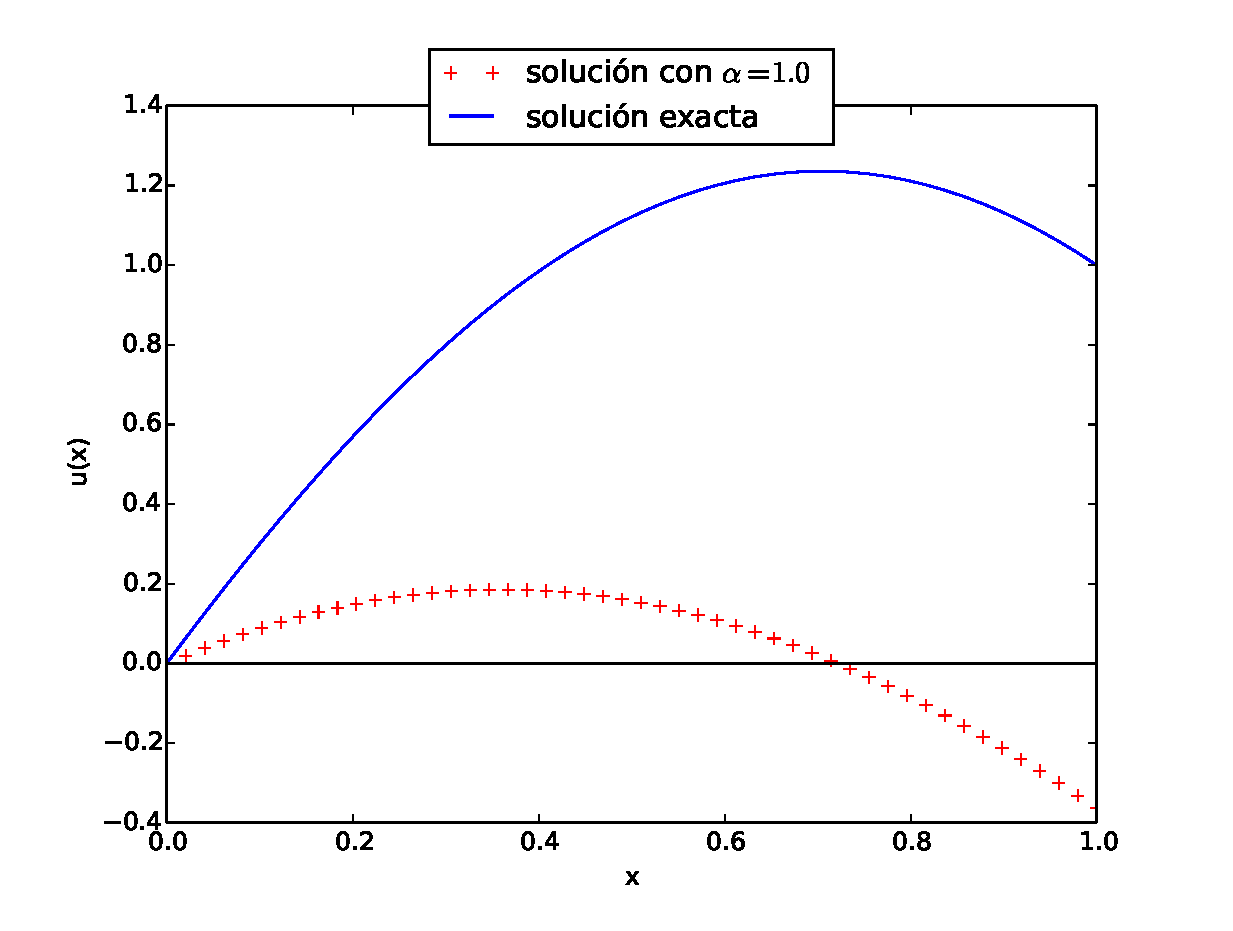
\includegraphics[scale=0.5]{MetodoDisparo2014_01.eps}
\end{figure}
\end{frame}
\begin{frame}[fragile]
\frametitle{Solución con $y0 = array([0.0,\alpha=4.0])$}
\begin{figure}
	\centering
	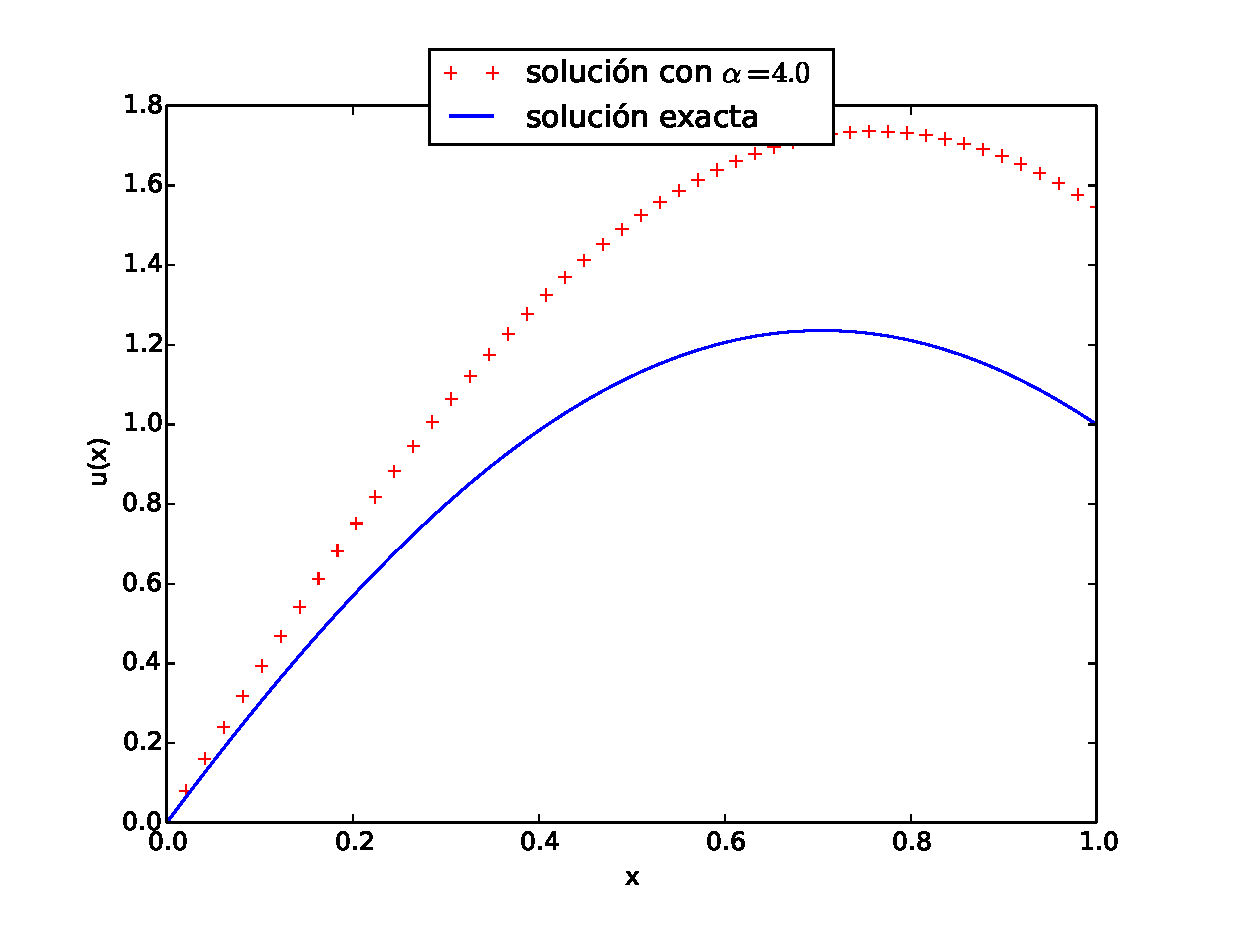
\includegraphics[scale=0.5]{MetodoDisparo2014_02.eps}
\end{figure}
\end{frame}
\begin{frame}
\frametitle{¿Qué hacemos?}
El siguiente paso es encontrar el valor de la raíz en donde $f(\alpha) = u_{\alpha}(1) - 1 = 0$.
\\
\medskip
Revisando los valores que obtenemos para $\alpha$:
\\
\medskip
$u_{1.0}(1) = -0.3633$ \\
$u_{4.0}(1) = 1.5464$
\\
\medskip
Por lo que necesariamente hay una raíz que debemos de utilizar para sustituirla en nuestro problema.
\end{frame}
\begin{frame}
El problema CVF se resuelve de manera exacta, la solución analítica es:
\begin{equation}
u(x) = \cos\left(\frac{x \pi}{2}\right) + 2 \sin \left(\frac{x \pi}{2}\right) -1
\end{equation}
\end{frame}
\begin{frame}[fragile]
\frametitle{Solución con $y0 = array([0.0,\alpha=??])$}
\begin{figure}
	\centering
	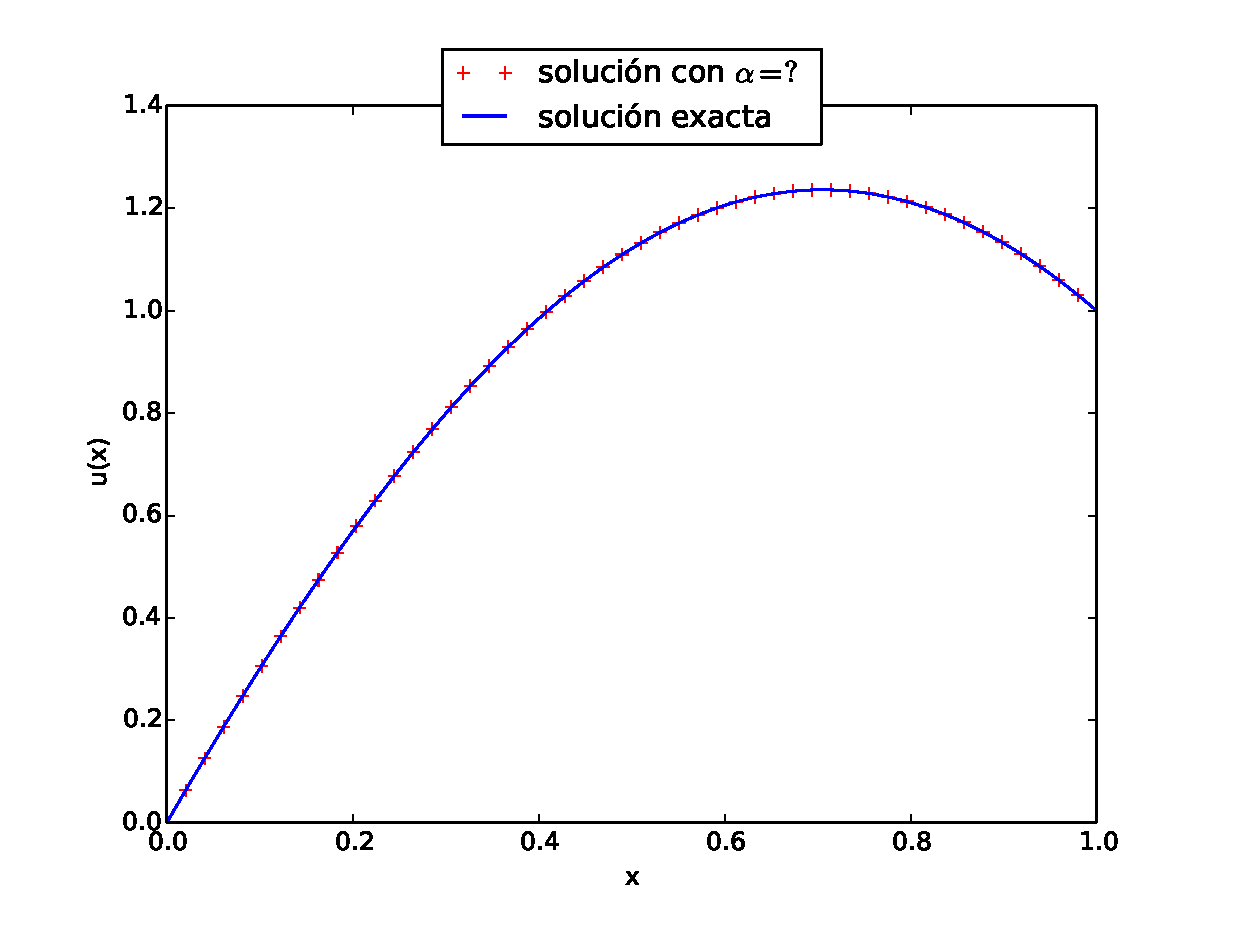
\includegraphics[scale=0.5]{MetodoDisparo2014_03.eps}
\end{figure}
\end{frame}
\end{document}